\documentclass[10pt]{beamer}

\usetheme{Frankfurt}
\useoutertheme{default}
\setbeamertemplate{footline}[page number]
\setbeamertemplate{navigation symbols}{} 

\usepackage{cmap}					% поиск в PDF
\usepackage[T2A]{fontenc}			% кодировка
\usepackage[utf8]{inputenc}			% кодировка исходного текста
\usepackage[english]{babel}	% локализация и переносы
\usepackage{indentfirst}
\usepackage{wrapfig}
\frenchspacing

\hypersetup{
	colorlinks=true,
	linkcolor=blue,
	filecolor=magenta,      
	urlcolor=cyan,
	pdfpagemode=FullScreen,
}

\title{Overview on the weather forecasting}
\date{\today}
\author{Kirill Semkin}

\institute[MIPT]{Intelligence systems department \\ MIPT}

\begin{document}
	
	\begin{frame}[c]
		\titlepage
	\end{frame}
	
	\begin{frame}{What is the weather}
		
		 \textit{Weather} is the state of the atmosphere at a specific time and place. The atmosphere works as a giant fluid system which transfers mass and energy around the globe. The fluid is a complex mixture, but the main components are air ($N_2, O_2$) and water vapour ($H_2 O$). The system is affected by the "external" forces: space (e.g. solar radiation) and the planet's surface (e.g. water sources, terrain heat, mountains). The overall dynamics are described by the fundamental laws of physics. 
		 
		 \vfill
		 \centering
		 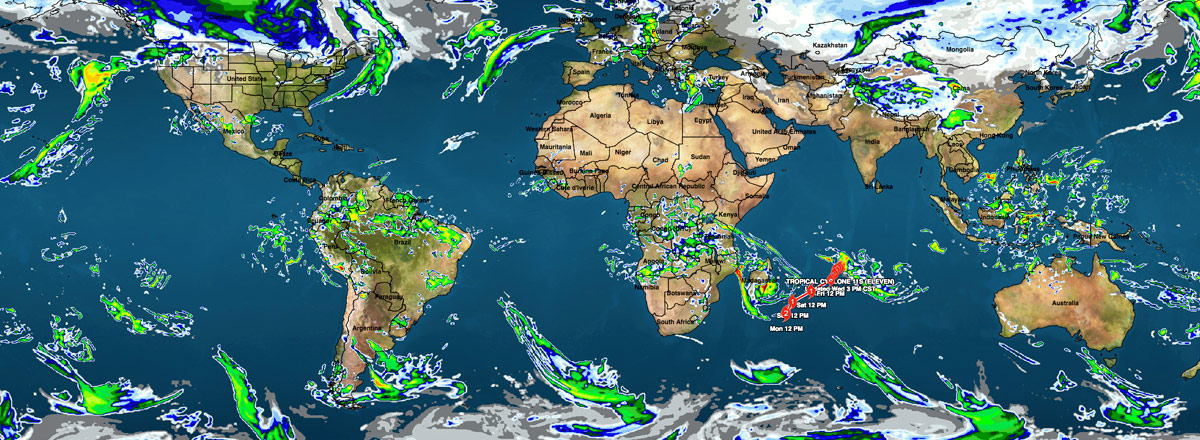
\includegraphics[height=0.4\textheight, keepaspectratio]{img/slide_global2}
		
	\end{frame}	
	
	\begin{frame}{The main variables}
		
		The weather can be characterized by its motion, thermodynamics, components' phase states.
		
		\begin{table}[h]
			\centering
			\label{tab:symbols}
			\begin{tabular}{|l|l|}
				\hline
				\textbf{Symbol} & \textbf{Meaning} \\
				\hline
				$(u, v, w)$ & Zonal, meridional, and vertical velocity components \\
				\hline
				$p$ & Pressure \\
				\hline
				$T$ & Temperature \\
				\hline
				$\Phi$ & Geopotential (related to gravitational potential energy) \\
				\hline
				$\rho$ & Air density \\
				\hline
				$q$ & Specific humidity \\
				\hline
				$f = 2\Omega \sin \phi$ & Coriolis parameter, depends on latitude $\phi$ \\
				\hline
				$R$ & Gas constant for dry air \\
				\hline
				$c_p$ & Specific heat at constant pressure \\
				\hline
			\end{tabular}
		\end{table}
		
	\end{frame}	
	
	\begin{frame}{Preliminaries to the Governing dynamics}
		
		\begin{enumerate}
			\item Every physical model has its limits. The chosen equations have to be adequate to the real observations.
			
			\item The equations must describe how the air masses are moved, how different types of energy are moved, and how proportions of different air components are changed.
			
			\item Introduce \textit{the material derivative}
			
			\begin{equation*}
				\frac{\mathrm{D}y}{\mathrm{D}t} \equiv \frac{\partial y}{\partial t} + \mathbf{u} \cdot \nabla y,
			\end{equation*}
			
			It basically corresponds to the total variation of $y$ in time if the $y$ is associated with the moving flow $u$. In our case $u$ will be the moving air masses.
		\end{enumerate}
		
	\end{frame}
	
	\begin{frame}{The Governing dynamics}
		
		\begin{enumerate}
			\item<only@1> The air in the atmosphere is quite sparse so we can use the \textbf{ideal gas} model as a state equation
			
			\begin{equation}
				p = \rho R T.
			\end{equation}
			
			\item<only@1> \textbf{Continuity Equation} describes mass conservation
			
			\begin{equation}
				\frac{D\rho}{Dt} + \rho \nabla \cdot \mathbf{v} = 0.
			\end{equation}
			
			\item<only@1> Because the atmosphere is thin, vertical acceleration is negligible, so we have balanced forces - \textbf{Hydrostatic balance}:
			
			\begin{equation}
				\frac{\partial p}{\partial z} = -\rho g.
			\end{equation}
			
			This links pressure and altitude — a key simplification in global models.
			
			\item<only@2> The horizontal acceleration of the masses is described by the \textbf{Navier–Stokes equations}. It is basically the Newtone's second law for viscous fluid
			
			\begin{align}
				\frac{Du}{Dt} - fv &= -\frac{1}{\rho} \frac{\partial p}{\partial x} + F_u, \\
				\frac{Dv}{Dt} + fu &= -\frac{1}{\rho} \frac{\partial p}{\partial y} + F_v,
			\end{align}
			
			where $F_u$, $F_v$ are frictional forces (like viscosity force = $\nu \Delta \boldsymbol{v}$, $\nu$ is kinetic viscosity).
			
			\item<only@2> \textbf{Thermodynamic Energy Equation} describes differential change of the heat in the "small" air parcel.
			
			\begin{equation}
				\frac{DT}{Dt} - \frac{1}{\rho \cdot c_p} \frac{Dp}{Dt} = \frac{Q}{c_p},
			\end{equation}
			
			where $Q$ is diabatic heating (radiation, latent heat, etc.). The diffusion term $\nabla \cdot (k \nabla T) $ is negligible relative to convection, work of expansion and external sources.
			
			\item<only@3> \textbf{Moisture Conservation}
			
			\begin{equation}
				\frac{Dq}{Dt} = S_q,
			\end{equation}
			
			where $S_q$ includes sources/sinks (condensation, evaporation, precipitation).
			
		\end{enumerate}
		
	\end{frame}
	
	\begin{frame}{Numerical integration - classical weather prediction}
		
		The basic computational scheme is:
		
		\begin{enumerate}
			\item The Earth is covered by the grid (Cubed-Sphere, Icosahedral).
			\item Apply finite differences to the derivatives (time and space)
			\item Set grid-specific boundary conditions and initial conditions from the meteostations, satellites, etc.
			\item Integrate forward
		\end{enumerate} 
		
		\begin{alertblock}{Do we have scheme's numerical approximation?}
			Typical size of the grid cell is 10-25 km (because of the enormous size of the equations' system). Not only do we have no guarantees for numerical convergence, but we also miss small-scale processes which are smaller than the grid cell. \textit{That's one reason why we don't have precise weather forecast}.
		\end{alertblock}
	
	\end{frame}
	
	\begin{frame}{Weather is a chaotic dynamical system}
		
		\only<1>{
			This is the second reason why accurate predicting is impossible. For illustration we will use classical \textit{Lorenz system}:
		}
		
		\only<1-2>{
		\begin{align*}
			\frac{dX}{dt} &= \sigma (Y - X), \\
			\frac{dY}{dt} &= X (\rho - Z) - Y, \\
			\frac{dZ}{dt} &= XY - \beta Z.
		\end{align*}
	}
		
		\only<1>{
			These equations can be derived from the previous physics laws using several simplifications. The variables here are:
			
			\begin{itemize}
				\item $X$: The rate of convection (how intensely the fluid is rolling). A positive $X$ means clockwise rotation, negative means counterclockwise.
				\item $Y$: The temperature difference between the ascending and descending fluid currents.
				\item $Z$: The distortion of the vertical temperature profile from linearity (how much the temperature graph deviates from a straight line).
			\end{itemize}
		}
		
		\only<2>{
			The parameters $\sigma$, $\rho$, and $\beta$ are dimensionless numbers related to the physical properties of the fluid:
			
			\begin{itemize}
				\item $\sigma$: The Prandtl number (ratio of viscous diffusion to thermal diffusion).
				\item $\rho$: The Rayleigh number (ratio of buoyancy to viscous forces), normalized by a critical value. This is the primary ``heating'' parameter.
				\item $\beta$: A geometric factor related to the aspect ratio of the convection cells.
			\end{itemize}
		}
		
		\only<3>{
			When $\rho=28, \sigma = 10, \beta = 8 / 3$ the Lorenz system has chaotic solutions (but not all solutions are chaotic). Almost all initial points will tend to an invariant set - the \textit{Lorenz attractor} – a strange fractal attractor. System's trajectories heavily depends on the initial conditions.
			
			\vfil
			\begin{figure}[h]
				\centering
				\href{https://commons.wikimedia.org/wiki/File:Lorenz_attractor_small.gif}{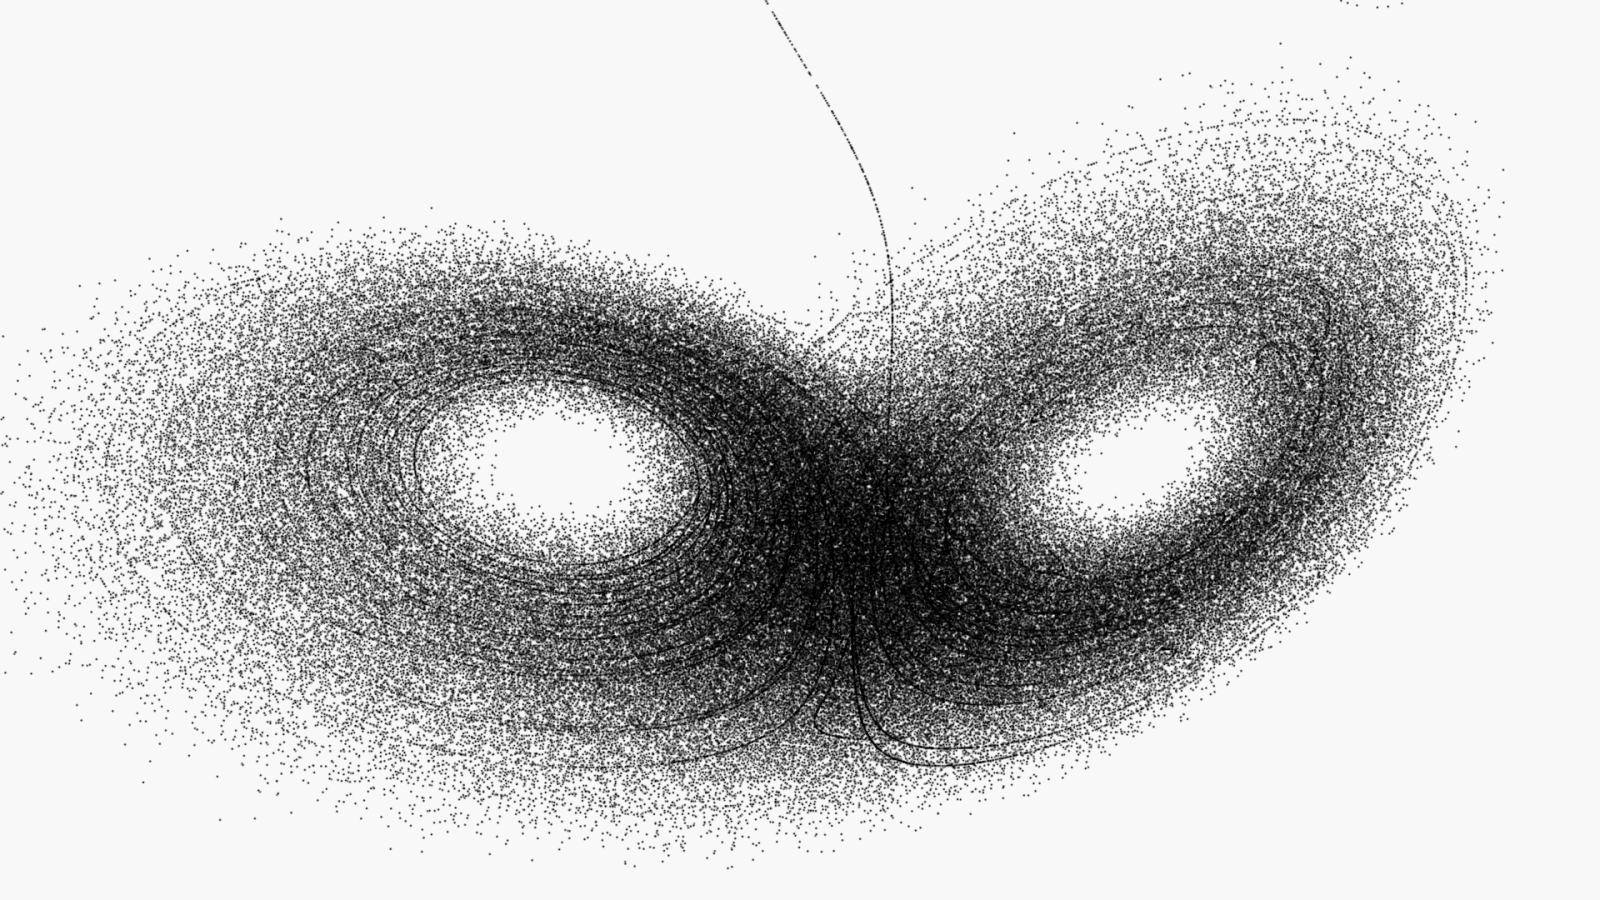
\includegraphics[width=0.7\textwidth, keepaspectratio]{img/Lorenz_attractor}}
				\caption{The Lorenz attractor}
			\end{figure}
		}
		
	\end{frame}
	
	\begin{frame}{Numerical integration - Parametrization}
		
		The small-scale processes such as
		
		\begin{enumerate}
			\item Individual clouds or raindrops,
			\item Turbulent eddies in the boundary layer,
			\item Vertical convection (thunderstorms, updrafts, downdrafts),
			\item Radiative transfer through clouds and gases,
			\item Surface fluxes of heat and moisture,
		\end{enumerate}
		
		can't be restored from the grid solution. These are crucial factors for the weather formation and can't be ignored. To embed them into the system we use \textit{parametrization} - replacing the explicit (unresolvable) physical process with a simplified, statistical, or empirical formula that expresses its average effect on the larger-scale (resolved) flow.
		
		\begin{exampleblock}{Example: Convective heating rate $Q_c$}
			 It describes vertical heat transfer by the clouds. For some function $f$, $Q_c$ can be approximated from the gird as
			
			\begin{equation*}
				 Q_c = f(T, q, p).
			\end{equation*}
			
		\end{exampleblock}
		
	\end{frame}
	
	\begin{frame}{ML models}
		
		Main idea - just solve regression problem for the physical variables using powerful models and large dataset.
		
		\begin{enumerate}
			\item \textit{Architectures}: RNN, CNN, Transformers
			\item \textit{Input}: Gridded atmospheric data at the current time (e.g., geopotential, temperature, wind at different heights)
			\item \textit{Output}: The same grid, but at 6, 12, 24 hours, etc. into the future
			
			\item \textit{Pros}: High forecast speed, high accuracy (short, mid-term)
			\item \textit{Cons}: Data dependence, difficulty with extreme events, long-term stability issues
		\end{enumerate}
		
		The \href{https://colab.research.google.com/drive/1dQ_V5-y1ieRqrpTG4po_Kx_D8NvZwRyK?usp=sharing\#scrollTo=srfsF01OLV-C}{demonstartion code} - ResNet for global temperature forecasting.
		
	\end{frame}
	
	\begin{frame}{Comparison of the approaches}
		
		\begin{table}[h]
			\centering
			\caption{Traditional vs. ML Approaches}
			\label{tab:comparison}
			\begin{tabular}{|p{0.25\textwidth}|p{0.3\textwidth}|p{0.3\textwidth}|}
				\hline
				\textbf{Criterion} & \textbf{Traditional Physical Models} & \textbf{Pure ML Models} \\
				\hline
				Basis & Physics equations & Historical data (reanalyses) \\
				\hline
				Speed & Slow (hours of computation) & Very fast (seconds/minutes) \\
				\hline
				Interpretability & High (physically based) & Low ("black box") \\
				\hline
				Accuracy & Very high, but with systematic errors & Comparable to or exceeds best models at medium ranges \\
				\hline
				Extreme event representation & Good, through physics & Data-dependent, may underestimate \\
				\hline
				Main cost & Computation (supercomputer) & Model training (very expensive), inference is cheap \\
				\hline
			\end{tabular}
		\end{table}
		
	\end{frame}
	
	\begin{frame}{PINNs: ML model $\to$ Classical}
		The ML model approximate solution function for some variable $\hat{u} = f(t, \boldsymbol{x})$. It learns by maximizing empirical risk function (like MSE) $\mathcal{L}_{\text{data}}$ on the data. We can regularize the risk using the discrepancy of $\hat{u}$ when substituted into the physics equations:
		
		\begin{equation*}
			\mathcal{L}_{\text{physics}} = \| g(u, \partial_t u, \nabla u, \ldots) \|^2 ,
		\end{equation*}
		
		where $g$ is the physics equations (Naive-Stocks, Thermodynamics, etc.). The final loss is a linear combination:
		
		\begin{equation}
			\mathcal{L} = \mathcal{L}_{\text{data}} + \lambda \mathcal{L}_{\text{physics}}
		\end{equation}
		
		The approach is very similar to the \href{https://en.wikipedia.org/wiki/Penalty_method}{\textit{penalty method}} in the constraint optimization.
		
		The demonstration on the \href{https://en.wikipedia.org/wiki/File:Lagrangian_trajectories_anumation_of_a_Taylor_Green_Vortex.gif}{Taylor-Green vortex} is \href{https://colab.research.google.com/drive/1UuzAmv43c6K9LmQ1cB4pSUPjrK1kqoHv?usp=sharing}{available}.
		
	\end{frame}
	
	\begin{frame}{Neural parametrizations: Classical $\to$ ML model}
		
		NNs can be used in the classical models as more accurate parametrization of sub-grid processes instead of hand-made heuristics. They also can adjust outputs of the classical models e.g. correcting temperature or precipitation probability for a specific location.
		
		\vfill
		Publications on the topic:
		\begin{enumerate}
			\item Beucler, T., Pritchard, M., Rasp, S., Ott, J., Baldi, P., and Gentine, P. (2021). \emph{Enforcing analytic constraints in neural networks for modeling physical processes with irregular outputs}. Journal of Advances in Modeling Earth Systems (JAMES), 13(2).
			
			\item Subramanian, S., Chattopadhyay, A., Gunzburger, M., and Balajewicz, M. (2023). \emph{Physics-informed neural networks for atmospheric dynamics}. Geoscientific Model Development (GMD), 16(3), 943–960.
		\end{enumerate}
		
	\end{frame}
	
	\begin{frame}{Current state of affairs: \href{https://sites.research.google/gr/weatherbench/}{WeatherBench}}
		\begin{figure}
			\centering
			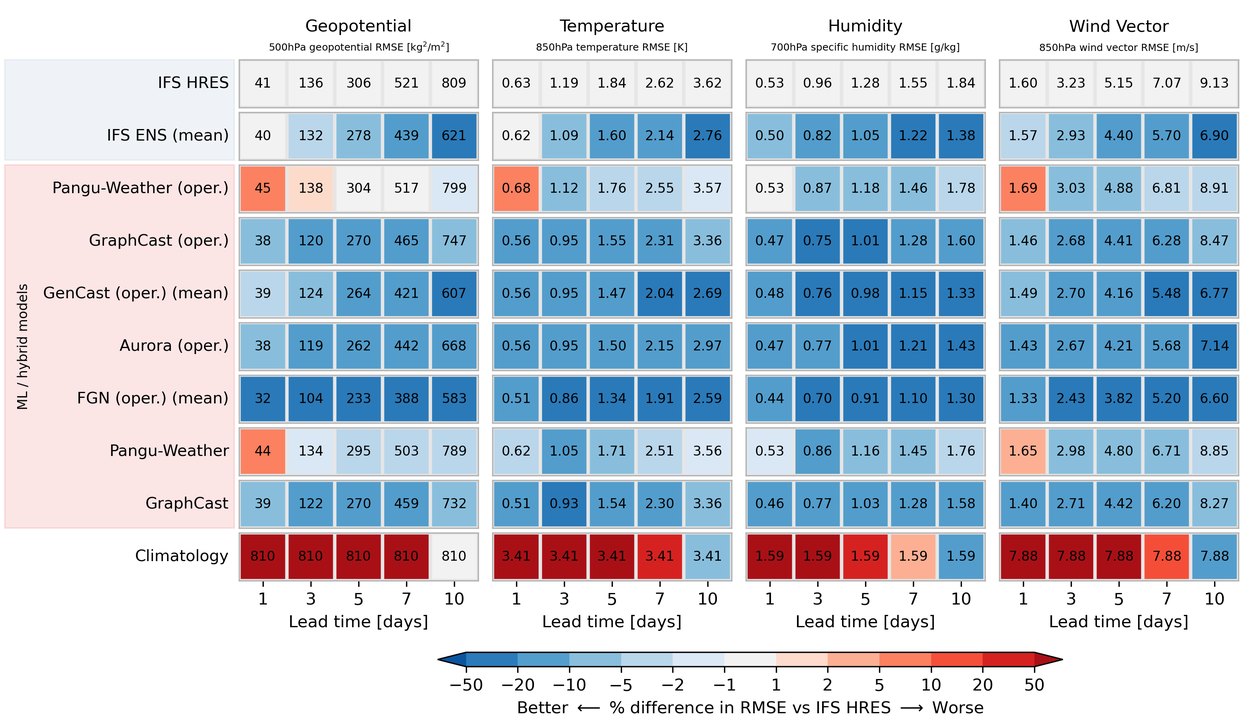
\includegraphics[width=\linewidth, keepaspectratio]{img/deterministic_upper_2022.width-1250}
			\caption{Models' metrics compared to the IFS model on different prediction tasks}
		\end{figure}
	\end{frame}

	
\end{document}